\documentclass[12pt,a4paper]{article}
\usepackage[utf8]{inputenc}
\usepackage[spanish]{babel}
\usepackage{amsmath,amssymb}
\usepackage{graphicx}
\usepackage[T1]{fontenc}
\usepackage{hyperref}
\hypersetup{
    bookmarks=true,
    breaklinks=true,
    colorlinks=true,
    linkcolor=blue,
    urlcolor=blue,
    citecolor=blue
}
\usepackage{xcolor}
\usepackage{booktabs}
\usepackage{fancyhdr}
\usepackage{longtable}
\usepackage{caption}
\usepackage{setspace}
\usepackage{array}
\usepackage[round]{natbib}
\bibliographystyle{apalike}

\usepackage[letterpaper,left=2.25cm,top=3.0cm,right=2.25cm,bottom=2.0cm, headsep=0.8cm, headheight=50pt]{geometry}

\newcommand{\NombreAlumno}{Junior Arturo Vázquez Leonel}
\newcommand{\Matricula}{2430319}
\newcommand{\NombreProyecto}{Lectura Analítica: Historia de la Inteligencia Artificial}
\newcommand{\NombreProyectoheader}{Fundamento de Inteligencia Artificial \\ Actividad 2: Lectura analítica | Historia de la IA}
\newcommand{\nasesorinstitucional}{Dr. Said Polanco Martagón}
\newcommand{\ncarrera}{Ingeniería en Tecnologías de la Información e Innovación Digital}
\newcommand{\fechaPortada}{\today}

\pagestyle{fancy}
\fancyhf{}
\fancyhead[C]{%
    \begin{tabular}{@{} m{0.2\textwidth} m{0.5\textwidth} m{0.2\textwidth} @{}}
        
\includegraphics[height=1.20cm]{figs/UTYP.png}
        &
        \centering
        \scriptsize{\NombreProyectoheader}
        &
        
\includegraphics[height=1.5cm]{figs/LogoUPV_2023.png}
    \end{tabular}
}
\cfoot{\thepage}
\renewcommand{\headrulewidth}{0.8pt}
\renewcommand{\footrulewidth}{0.4pt}

\addto\captionsspanish{
  \renewcommand{\tablename}{Tabla}
  \renewcommand{\listtablename}{Índice de Tablas}
}

\newcolumntype{C}[1]{>{\centering\arraybackslash}p{#1}}

\setstretch{1.3}

\begin{document}

\begin{titlepage}
\vspace*{-2cm}
\begin{center}
\begin{tabular}{cC{6cm}c}

\includegraphics[height=2.25cm]{figs/UTYP.png} & 
& 
\includegraphics[height=2.25cm]{figs/LogoUPV_2023.png}   \\
\end{tabular} \\[0.5cm]

{\Large \textbf{UNIVERSIDAD POLITÉCNICA DE VICTORIA}}\\[1.0cm]

{\Large \textbf{REPORTE DE ACTIVIDADES}}\\[0.75cm]

{\Large \textbf{\MakeUppercase{\NombreProyecto}}}\\[1.0cm]

QUE PRESENTA

\textbf{\MakeUppercase{\NombreAlumno}}\\[0.5cm]
\textbf{MATRÍCULA: \Matricula}\\[1.0cm]

COMO PARTE DE LA ASIGNATURA DE\\
\textbf{FUNDAMENTOS DE INTELIGENCIA ARTIFICIAL}\\[0.5cm]
DE LA CARRERA DE\\
\textbf{\MakeUppercase{\ncarrera}}\\[0.75cm]

PROFESOR:\\
\textbf{\MakeUppercase{\nasesorinstitucional}}\\[0.5cm]

\end{center}
\begin{flushright}
\vfill
Ciudad Victoria, Tamaulipas, \fechaPortada.
\end{flushright}
\end{titlepage}

\tableofcontents
\newpage

\section{Introducción}

La Inteligencia Artificial (IA) constituye uno de los campos de investigación más transformadores y multidisciplinarios en la historia de la ciencia y la tecnología. Desde sus fundamentos teóricos en la lógica matemática y la teoría de la computación hasta su manifestación contemporánea en sistemas de aprendizaje profundo y modelos generativos, la IA ha transitado por un camino marcado por ciclos de optimismo desbordante, estancamiento crítico y renacimiento tecnológico \citep{haenlein2019}.

El presente reporte técnico tiene como objetivo realizar un análisis exhaustivo de la evolución histórica de la Inteligencia Artificial, examinando los hitos fundamentales que han definido cada etapa de su desarrollo. Este análisis se estructura de manera cronológica, partiendo de las bases teóricas establecidas por Alan Turing y los pioneros de la computación, atravesando los períodos de auge y declive conocidos como ``primaveras'' e ``inviernos'' de la IA, hasta llegar a la era actual dominada por el Deep Learning, la IA generativa y las arquitecturas embebidas como TinyML.

La relevancia de este estudio radica en la necesidad de comprender cómo los avances teóricos, algorítmicos y computacionales han convergido para hacer posible la implementación de sistemas inteligentes que antes eran computacionalmente inviables. Como señala \citet{buchanan2005}, la historia de la IA no es simplemente una cronología de logros técnicos, sino un reflejo de la evolución del pensamiento humano sobre la naturaleza de la inteligencia y la posibilidad de replicarla en máquinas.

Desde la perspectiva de la Ingeniería en Tecnologías de la Información e Innovación Digital, el análisis de la historia de la IA proporciona un marco conceptual indispensable para entender el estado actual del campo y proyectar sus tendencias futuras. La intersección entre los lenguajes de programación predominantes en cada época (LISP, Prolog, Python, C++), las capacidades de hardware disponibles y los paradigmas algorítmicos vigentes ha definido la trayectoria de la disciplina y las aplicaciones que hoy consideramos cotidianas \citep{gill2022}.

Este documento se organiza en las siguientes secciones: primero, un desarrollo cronológico y técnico de los hitos fundamentales de la IA, integrando la relación con los lenguajes de programación y paradigmas computacionales de cada época; segundo, un análisis crítico del hardware y su rol como habilitador ---y en ciertos periodos, como limitante--- del progreso en IA; tercero, una exploración de la transición hacia el Deep Learning, la IA generativa y las arquitecturas embebidas; y finalmente, conclusiones que sintetizan los hallazgos del análisis.

\section{Desarrollo Cronológico y Técnico de la Inteligencia Artificial}

La historia de la Inteligencia Artificial puede estructurarse en etapas diferenciadas, cada una caracterizada por paradigmas teóricos, lenguajes de programación dominantes, logros emblemáticos y desafíos específicos. A continuación se presenta un recorrido integrado que vincula los hitos fundamentales con el ecosistema tecnológico de cada época.

\subsection{Antecedentes Filosóficos y Precursores Teóricos (Antes de 1950)}

Los antecedentes de la IA se remontan a la filosofía clásica, donde pensadores como Aristóteles formularon las bases de la lógica formal. Sin embargo, el primer paso concreto hacia la formalización del pensamiento como proceso mecánico fue dado por \textbf{René Descartes}, quien en el siglo XVII estableció la distinción entre mente y materia. Como analiza \citet{abramson2011}, la influencia cartesiana fue determinante en la formulación del Test de Turing, pues Turing heredó de Descartes la pregunta fundamental: ¿puede una máquina exhibir un comportamiento indistinguible del pensamiento humano?

En el siglo XIX, \textbf{Ada Lovelace} formuló la ``objeción de Lovelace'': las máquinas solo pueden hacer aquello para lo cual han sido programadas y no pueden originar nada nuevo. Esta objeción sigue siendo relevante en la era de la IA generativa \citep{natale2022}. En 1936, \textbf{Alan Turing} introdujo la \textit{Máquina de Turing} en su artículo ``On Computable Numbers'', formalizando la noción de ``algoritmo'' y estableciendo los límites teóricos de la computabilidad \citep{milkowski2022}.

\subsection{El Test de Turing y la Formalización de la Inteligencia (1950)}

En 1950, Turing publicó ``Computing Machinery and Intelligence'' en la revista \textit{Mind}, donde propuso reformular la pregunta ``¿pueden pensar las máquinas?'' por una más operativa mediante el \textbf{Juego de Imitación} (Test de Turing) \citep{turing1950}. Como analiza \citet{milkowski2022}, el Test no pretendía ser una definición formal de inteligencia, sino un ejercicio de \textit{ingeniería conceptual}: una herramienta para legitimar la discusión científica sobre la mecanización del pensamiento.

Es importante señalar que \citet{abramson2011} demuestra que Turing no era un conductista estricto. El Test establece una condición \textit{suficiente} ---pero no necesaria--- para la inteligencia. Además, \citet{buchanan2012} argumenta que la visión de Turing iba más allá del test: su concepto de la ``máquina infantil'' (\textit{child machine}) ---un sistema que aprende gradualmente mediante interacción con su entorno--- prefiguró los principios del aprendizaje automático moderno.

\subsection{El Nacimiento Formal de la IA y la Era Simbólica (1956--1974)}

El término ``Inteligencia Artificial'' fue acuñado en 1956 cuando \textbf{John McCarthy}, \textbf{Marvin Minsky}, \textbf{Nathaniel Rochester} y \textbf{Claude Shannon} organizaron el \textit{Dartmouth Summer Research Project on Artificial Intelligence} \citep{haenlein2019, mccarthy2006}. El primer paradigma dominante fue la \textbf{IA simbólica} (GOFAI, \textit{Good Old-Fashioned AI}), basada en la manipulación de símbolos y reglas lógicas.

\begin{figure}[htbp]
    \centering
    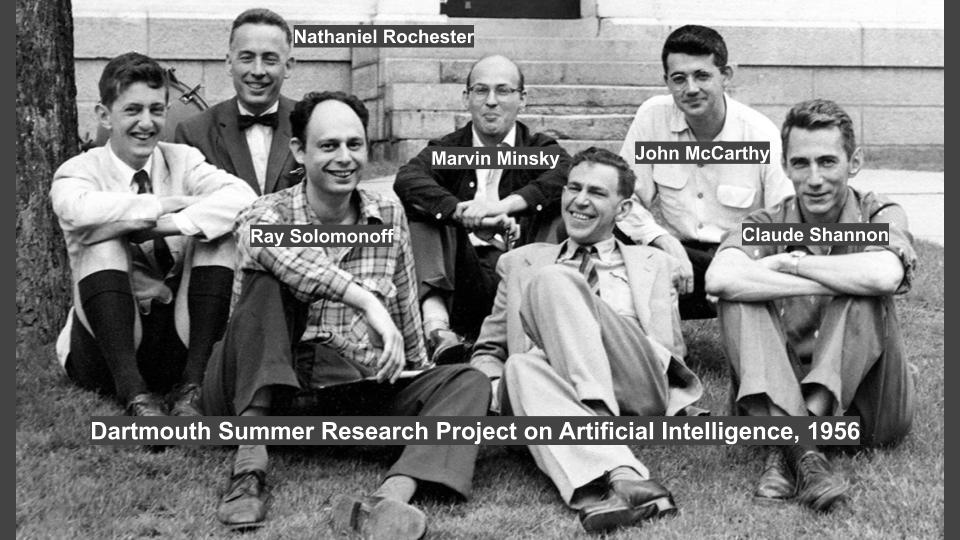
\includegraphics[width=0.75\textwidth]{figs/dartmouth_conference.jpg}
    \caption{Pioneros y fundadores en los inicios de la Inteligencia Artificial.}
    \label{fig:pioneros}
\end{figure}

En 1958, McCarthy creó \textbf{LISP} (List Processing), diseñado para procesamiento simbólico, con características revolucionarias como homoiconicidad, recolección automática de basura y evaluación dinámica. LISP se convirtió en el lenguaje estándar de la IA durante tres décadas e incluso dio lugar a hardware especializado (``máquinas LISP'').

Entre los logros más destacados de esta primera primavera:

\begin{enumerate}
    \item \textbf{Logic Theorist (1956):} De Newell, Shaw y Simon; primer programa capaz de demostrar teoremas del \textit{Principia Mathematica}.
    \item \textbf{General Problem Solver (1957):} Solucionador universal basado en análisis medios-fines \citep{haenlein2019}.
    \item \textbf{ELIZA (1964--1966):} De Joseph Weizenbaum (MIT); primer chatbot de procesamiento de lenguaje natural. Reveló que los usuarios atribuían comprensión y empatía a la máquina \citep{natale2022}.
    \item \textbf{DENDRAL (mediados de 1960s):} Primer sistema experto exitoso, para inferencia de estructuras moleculares \citep{buchanan2005}.
\end{enumerate}

En 1970, Minsky predijo que una máquina con inteligencia humana se desarrollaría en ``tres a ocho años'' \citep{haenlein2019}. Este optimismo desbordante preparó el terreno para la decepción posterior.

\subsection{Los Inviernos de la IA y sus Causas Técnicas (1974--1993)}

\subsubsection{Primer Invierno (1974--1980)}

En 1973, el \textbf{Informe Lighthill} cuestionó las promesas de la IA, argumentando que las máquinas solo alcanzarían el nivel de un ``aficionado experimentado''. Como consecuencia, el gobierno británico eliminó el financiamiento en IA en todas las universidades excepto Edinburgh, Sussex y Essex; Estados Unidos siguió el ejemplo recortando los fondos de DARPA \citep{haenlein2019}.

\subsubsection{Resurgimiento y Segundo Invierno (1980--1993)}

La IA resurgió en los 1980s con los \textbf{sistemas expertos} (reglas ``si-entonces''), como MYCIN (diagnóstico médico, Stanford) y R1/XCON (configuración de hardware, CMU/DEC). En 1972, \textbf{Prolog} (Programming in Logic) introdujo la programación declarativa basada en lógica de predicados, adoptado por el Proyecto de Quinta Generación de Japón.

\begin{table}[htbp]
    \centering
    \caption{Sistemas Expertos Relevantes en la Historia de la IA.}
    \label{tab:sistemas_expertos}
    \begin{tabular}{@{}llC{5.5cm}l@{}}
        \toprule
        \textbf{Sistema} & \textbf{Año} & \textbf{Función} & \textbf{Institución} \\ \midrule
        DENDRAL & 1965 & Inferencia de estructuras moleculares & Stanford \\
        MYCIN & 1976 & Diagnóstico de infecciones bacterianas & Stanford \\
        PROSPECTOR & 1978 & Exploración geológica & SRI International \\
        R1/XCON & 1980 & Configuración de sistemas VAX & CMU / DEC \\
        CADUCEUS & 1982 & Diagnóstico médico (500+ enfermedades) & Univ. Pittsburgh \\ \bottomrule
    \end{tabular}
\end{table}

Sin embargo, el segundo invierno (1987--1993) llegó cuando se evidenciaron las limitaciones de la IA simbólica: el \textit{problema del marco}, el cuello de botella de la adquisición del conocimiento, la explosión combinatoria, la fragilidad ante entradas ruidosas, y el colapso del mercado de hardware LISP \citep{haenlein2019}.

\subsection{El Auge del Machine Learning y la Era de Python (1986--2012)}

El renacimiento de la IA fue impulsado por un cambio paradigmático: la transición de la representación explícita del conocimiento hacia el \textbf{aprendizaje a partir de datos} \citep{lecun2015}.

\subsubsection{El Renacimiento Conexionista}

En 1986, Rumelhart, Hinton y Williams publicaron el algoritmo de \textbf{retropropagación}, que permitía entrenar redes neuronales multicapa. Las ideas conexionistas ya habían sido planteadas antes: el \textbf{Aprendizaje Hebbiano} (1949) propuso que las conexiones sinápticas se fortalecen con la activación simultánea, y el \textbf{Perceptrón de Rosenblatt} (1958) fue el primer modelo de red neuronal capaz de aprender, aunque Minsky y Papert demostraron sus limitaciones en 1969 \citep{haenlein2019}.

\subsubsection{Python y la Democratización del Machine Learning}

A partir del año 2000, \textbf{Python} se consolidó como herramienta dominante gracias a su simplicidad sintáctica, su ecosistema de bibliotecas (\texttt{NumPy}, \texttt{scikit-learn}, \texttt{TensorFlow}, \texttt{PyTorch}) y su interoperabilidad con backends en C/C++ y CUDA.

\subsubsection{Hitos Clave del Período}

\begin{enumerate}
    \item \textbf{Deep Blue vs. Kasparov (1997):} IBM Deep Blue procesaba 200 millones de posiciones/segundo y derrotó al campeón mundial \citep{haenlein2019}.
    \item \textbf{SVM (1990s):} Las Máquinas de Vectores de Soporte de Vapnik se convirtieron en el estándar para clasificación.
    \item \textbf{IBM Watson en Jeopardy! (2011):} Combinó NLP y aprendizaje automático para derrotar a campeones humanos \citep{buchanan2012}.
\end{enumerate}

\begin{table}[htbp]
    \centering
    \caption{Relación entre paradigmas de IA, lenguajes de programación y períodos históricos.}
    \label{tab:paradigmas_lenguajes}
    \begin{tabular}{@{}C{2.5cm}C{2.2cm}C{3.5cm}C{5cm}@{}}
        \toprule
        \textbf{Período} & \textbf{Lenguaje} & \textbf{Paradigma de IA} & \textbf{Aplicaciones Representativas} \\ \midrule
        1958--1980 & LISP & IA Simbólica, Búsqueda heurística & GPS, ELIZA, SHRDLU \\
        1972--1990 & Prolog & Programación lógica & Proyecto 5\textsuperscript{a} Gen., NLP \\
        1990--2010 & C/C++, MATLAB & ML estadístico, SVM & Deep Blue, robótica \\
        2010--presente & Python, C++ & Deep Learning, IA Generativa & AlphaGo, GPT, DALL-E \\
        2019--presente & C/C++, MicroPython & TinyML, Edge AI & IoT inteligente \\ \bottomrule
    \end{tabular}
\end{table}

\subsection{De Big Data a la Era del Cloud y Edge Computing (2005--presente)}

La explosión de datos generados por internet y redes sociales a partir de 2005 inauguró la era del \textbf{Big Data}. Por primera vez, los investigadores disponían de la materia prima masiva necesaria para entrenar modelos complejos. Sin embargo, procesar esta cantidad de información requirió una nueva infraestructura.

En la década de 2010, el \textbf{Cloud Computing} democratizó el acceso al cómputo de alto rendimiento. Empresas y universidades ya no necesitaban construir supercomputadoras físicas; podían alquilar clústeres de GPUs en la nube para entrenar algoritmos masivos. Más recientemente, la tendencia se ha expandido hacia el \textbf{Edge Computing} (cómputo en el borde), buscando llevar esa capacidad de procesamiento directamente a los dispositivos locales (teléfonos, sensores) para reducir la latencia y proteger la privacidad.

\begin{figure}[htbp]
    \centering
    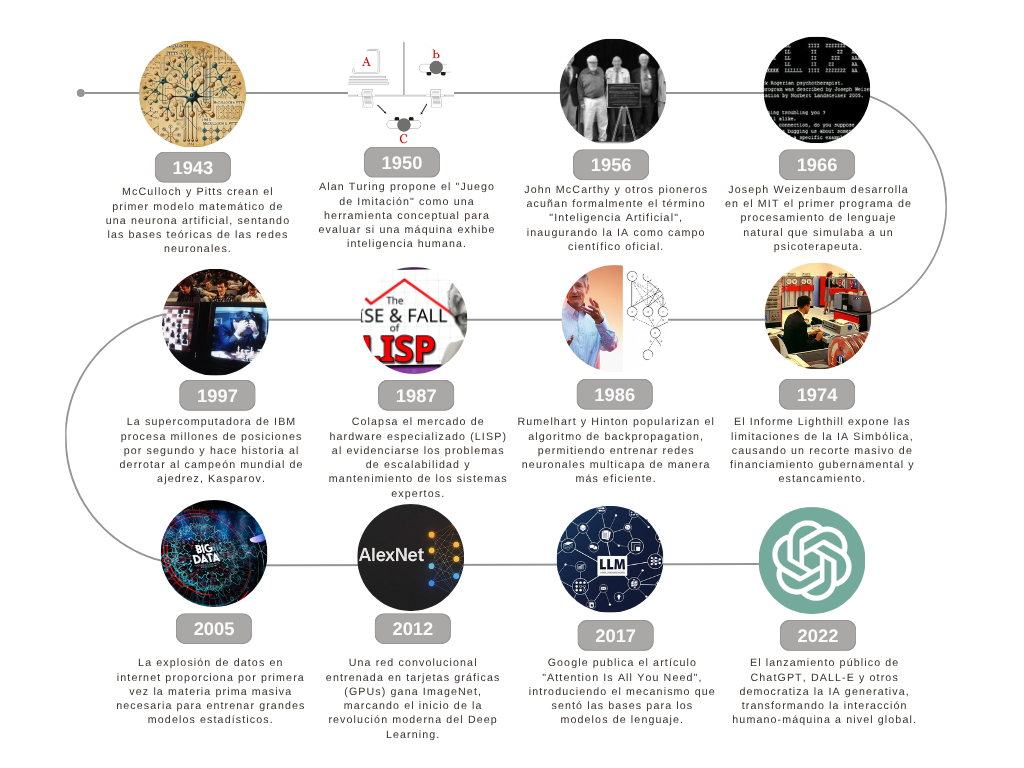
\includegraphics[width=\textwidth]{figs/linea_del_tiempo_IA.png}
    \caption{Línea de tiempo de los hitos fundamentales en la evolución cronológica y técnica de la IA.}
    \label{fig:timeline}
\end{figure}

\section{Análisis Crítico de Hardware: Cómputo como Habilitador y Limitante}

El progreso de la Inteligencia Artificial ha estado ligado a la evolución del hardware. A menudo, las ideas teóricas precedieron por décadas a las capacidades necesarias para implementarlas \citep{moore1965}.

\subsection{Ley de Moore y GPUs}
El verdadero punto de inflexión fue la adopción de las \textbf{Unidades de Procesamiento Gráfico (GPUs)}. Su paralelismo masivo resultó excepcional para las operaciones matriciales de las redes neuronales. Este hito se cristalizó en 2012 cuando \textbf{AlexNet}, entrenada en GPUs NVIDIA, arrasó en la competencia ImageNet \citep{krizhevsky2012}. 

\begin{figure}[htbp]
    \centering
    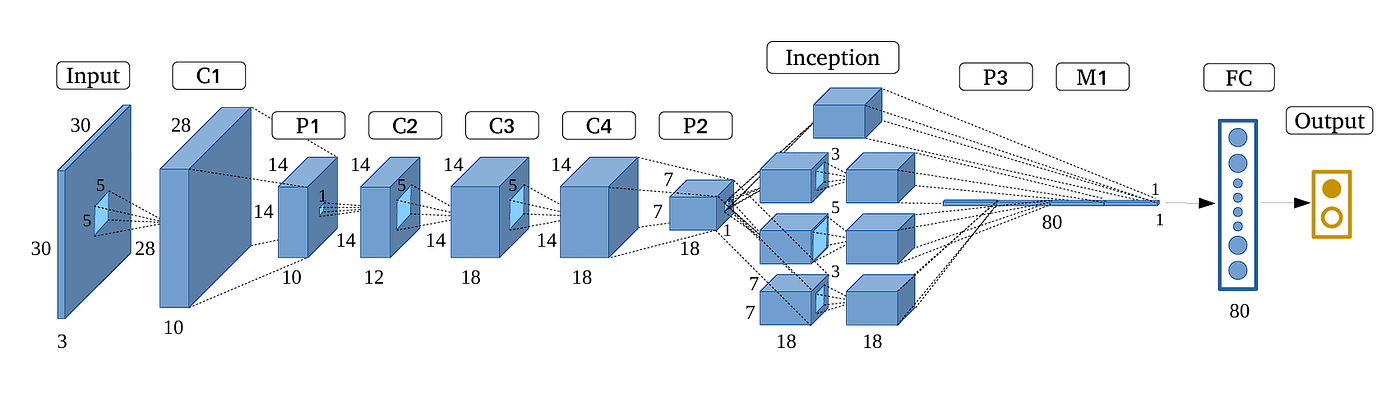
\includegraphics[width=0.85\textwidth]{figs/alexnet.png}
    \caption{Arquitectura de la red neuronal convolucional AlexNet (2012), cuyo entrenamiento en GPUs revolucionó el campo del Deep Learning.}
    \label{fig:gpu}
\end{figure}
Ante la creciente demanda, surgieron arquitecturas especializadas como las \textbf{TPUs (Tensor Processing Units)} de Google, diseñadas para operaciones tensoriales eficientes en inferencia y entrenamiento \citep{gill2022}, así como diversos ASICs y FPGAs orientados a IA.

\begin{table}[htbp]
    \centering
    \caption{Comparativa de hardware para entrenamiento e inferencia de IA.}
    \label{tab:hardware}
    \begin{tabular}{@{}C{2.5cm}C{2.5cm}C{3cm}C{4.5cm}@{}}
        \toprule
        \textbf{Plataforma} & \textbf{Rendimiento} & \textbf{Eficiencia Energética} & \textbf{Caso de Uso Principal} \\ \midrule
        CPU (Xeon) & Moderado & Moderada & Inferencia ligera, preprocesamiento \\
        GPU (A100) & Muy Alto & Alta & Entrenamiento de modelos grandes \\
        TPU (Google) & Extremo & Muy alta & Entrenamiento a escala de clústeres \\
        MCU (TinyML) & Bajo & Máxima & Inferencia en dispositivos embebidos \\ \bottomrule
    \end{tabular}
\end{table}

\subsection{Desfase entre Teoría y Práctica}
Un patrón recurrente es que las ideas teóricas superan temporalmente al hardware: el perceptrón (1958) y la retropropagación (1986) requirieron GPUs modernas para volverse redes profundas; el aprendizaje por refuerzo teórico de los 80s necesitó cómputo masivo para sistemas como AlphaGo (2016) \citep{silver2016}; y las GANs (2014) \citep{goodfellow2014} o los Transformers (2017) exigen millones de dólares en cómputo \citep{gill2022}.

\section{Transición del Machine Learning al Deep Learning y IA Generativa}

\subsection{De Machine Learning a la Revolución del Deep Learning}

Durante la década de los 90s y los primeros años del 2000, el \textbf{Machine Learning (Aprendizaje Automático)} clásico dominó el campo. Algoritmos como las Máquinas de Vectores de Soporte (SVM), los árboles de decisión y los modelos probabilísticos lograron grandes avances en predicción y clasificación estadística. Sin embargo, su limitación principal radicaba en que dependían fuertemente de la \textit{ingeniería de características} manual (feature engineering): requerían que un experto humano diseñara la representación de los datos para que el algoritmo pudiera entenderlos.

A partir de 2012, el enfoque hizo una transición profunda hacia el \textbf{Deep Learning}. A diferencia del Machine Learning clásico, el Deep Learning automatiza la extracción de características, utilizando redes neuronales artificiales de múltiples capas que aprenden por sí mismas las representaciones jerárquicas a partir de datos crudos. Entre sus arquitecturas fundamentales destacan:

\begin{figure}[htbp]
    \centering
    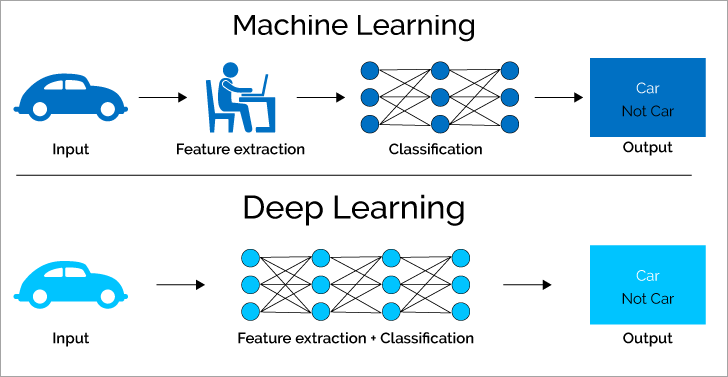
\includegraphics[width=0.75\textwidth]{figs/machine_learning_vs_deep_learning.png}
    \caption{Diferencia conceptual entre el enfoque clásico de Machine Learning y el de Deep Learning.}
    \label{fig:ml_vs_dl}
\end{figure}

\begin{itemize}
    \item \textbf{CNNs (Redes Convolucionales):} Diseñadas para datos con topología de cuadrícula (imágenes), utilizan filtros convolucionales para extraer jerarquías espaciales (bordes, texturas, formas) de manera automática \citep{lecun2015}.
    \item \textbf{RNNs (Redes Recurrentes):} Procesan datos secuenciales (como series de tiempo) manteniendo una memoria interna de pasos temporales previos mediante funciones de activación que combinan las entradas actuales con el contexto histórico.
    \item \textbf{LSTMs (Long Short-Term Memory):} Una variante de las RNNs diseñada para mitigar la pérdida de memoria a largo plazo mediante mecanismos matemáticos que deciden de forma autónoma qué información retener, olvidar o actualizar.
\end{itemize}

\subsection{La Arquitectura Transformer y los LLMs}

En 2017, \citet{vaswani2017} introdujeron el \textbf{Transformer}, prescindiendo por completo de la estructura de procesamiento secuencial en favor de los \textit{mecanismos de atención}.

\subsubsection{El Mecanismo de Atención}

Este mecanismo calcula estadísticamente la relevancia de todos los elementos de una secuencia simultáneamente, permitiendo al modelo enfocar su ``atención'' en las partes más importantes del contexto, independientemente de la distancia entre las palabras. Esta arquitectura permite una paralelización masiva y catalizó el desarrollo de los Modelos de Lenguaje a Gran Escala (LLMs). Modelos como BERT (Google) y la serie GPT (OpenAI) revolucionaron el procesamiento de lenguaje natural \citep{gill2022}.

\begin{table}[htbp]
    \centering
    \caption{Evolución de modelos Transformer representativos.}
    \label{tab:llms}
    \begin{tabular}{@{}llrl@{}}
        \toprule
        \textbf{Modelo} & \textbf{Organización} & \textbf{Parámetros} & \textbf{Año} \\ \midrule
        BERT & Google & 340 M & 2018 \\
        GPT-3 & OpenAI & 175 B & 2020 \\
        GPT-4 & OpenAI & $\sim$1.76 T & 2023 \\
        LLaMA 2 & Meta & 7--70 B & 2023 \\ \bottomrule
    \end{tabular}
\end{table}

\subsection{IA Generativa: Más Allá del Texto}

La \textbf{IA generativa} crea contenido nuevo (texto, imágenes, código) a partir de patrones aprendidos. Los principales paradigmas incluyen VAEs (Autoencoders Variacionales), GANs (Redes Adversariales), Modelos de Difusión (DALL-E, Stable Diffusion) y Modelos Autorregresivos (LLMs). Como señala \citet{natale2022}, es crucial distinguir entre esta generación estadística de alta calidad y la creatividad humana genuina, evitando el ``efecto Lovelace''.

\begin{figure}[htbp]
    \centering
    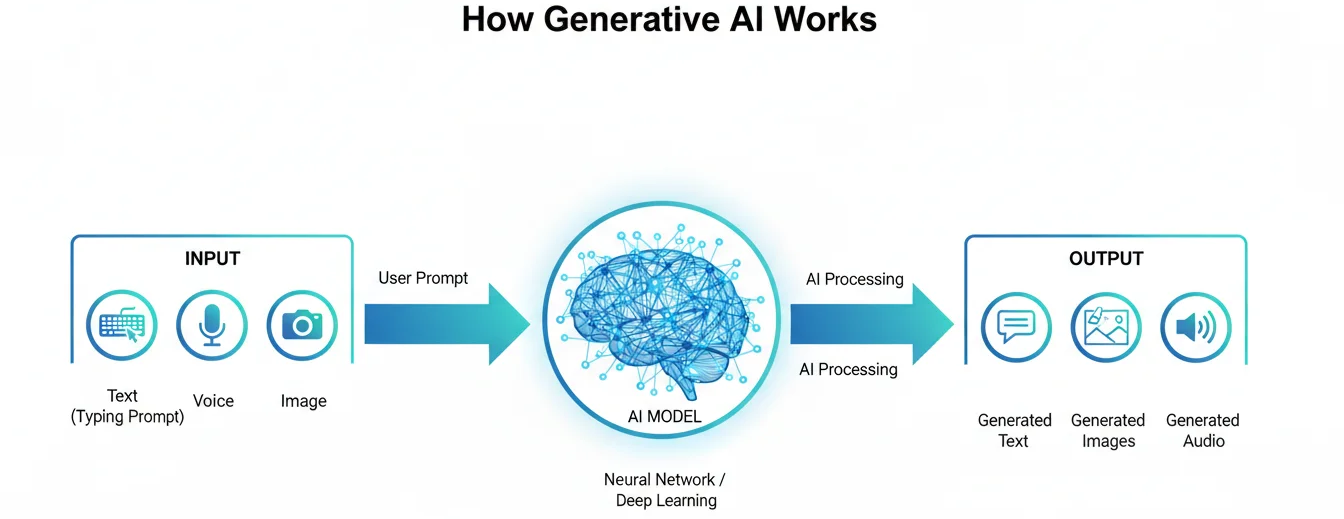
\includegraphics[width=0.85\textwidth]{figs/how-generative-ai-works.png}
    \caption{Las arquitecturas generativas actuales permiten sintetizar imágenes realistas o artísticas a partir de descripciones textuales.}
    \label{fig:generativa_img}
\end{figure}

\subsection{TinyML: Inteligencia Artificial en el Borde}

\textbf{TinyML} lleva el aprendizaje automático a microcontroladores y dispositivos embebidos con recursos mínimos (menos de 1~MB RAM, milivatios de consumo) \citep{warden2019, banbury2021}. Permite la inferencia local sin conexión a la nube, reduciendo la latencia y protegiendo la privacidad de los datos.

\begin{figure}[htbp]
    \centering
    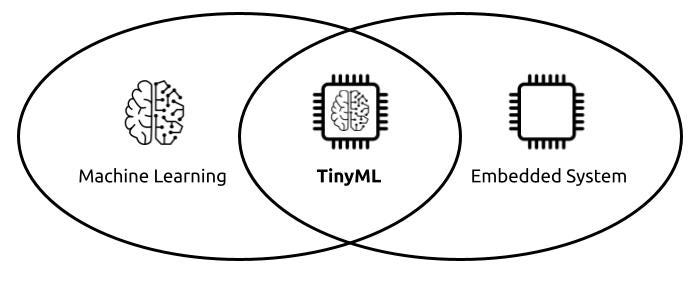
\includegraphics[width=0.75\textwidth]{figs/tinyML.jpg}
    \caption{Diagrama conceptual de TinyML como la intersección directa entre las técnicas de Machine Learning y los Sistemas Embebidos.}
    \label{fig:tinyml_board}
\end{figure}

Para adaptar los modelos, TinyML emplea técnicas como:
\begin{enumerate}
    \item \textbf{Cuantización:} Reducción de precisión (ej. de 32 a 8 bits).
    \item \textbf{Poda (\textit{Pruning}):} Eliminación de pesos cercanos a cero.
    \item \textbf{Destilación:} Un modelo pequeño imita a uno grande.
\end{enumerate}

\begin{table}[htbp]
    \centering
    \caption{Aplicaciones representativas de TinyML en dispositivos embebidos.}
    \label{tab:tinyml}
    \begin{tabular}{@{}C{3cm}C{3cm}C{6cm}@{}}
        \toprule
        \textbf{Aplicación} & \textbf{Hardware} & \textbf{Descripción} \\ \midrule
        Wake Word Detection & Arduino Nano 33 BLE & Detección de palabras clave en el dispositivo \\
        Detección de anomalías & ESP32 & Monitoreo predictivo de maquinaria industrial \\
        Reconocimiento de gestos & STM32 & Interpretación de gestos manuales para interfaces \\
        Visión por computadora & Arduino Nicla Vision & Detección de objetos en tiempo real con cámara \\ \bottomrule
    \end{tabular}
\end{table}

La convergencia de TinyML con el Internet de las Cosas (IoT) y las redes 5G promete democratizar aún más el acceso a la IA, llevando capacidades de inferencia inteligente a miles de millones de dispositivos. Esta tendencia representa un cambio fundamental: de un modelo centralizado en la nube a un modelo distribuido e inteligente en el borde.

\section{Conclusiones}

La historia de la INteligencia Artificial nos ha demostrado que esta misma no ha sido lineal, sino que han habido ciclos determinados muy marcados gracias a tres factores esenciales: Las innovaciones teóricas y algorítmicas, la disponibilidad del Big Data, y la evolución exponencial de la capacidad del hardware, como las gráficas NVIDIA.

Los hitos analizados en este reporte nos demuestran que existieron diversos periodos de estancamiento o también llamados inviernos los cuales ocurrieron debido a que la ambición de las promesas superó la viabilidad tecnológica. Y por el contrario, gracias a el aumento del hardware de calidad como las GPUs hubo una gran aceleración maduración de los paradigmas algorítmicos.

Actualmente, la transición del Machine Learning hacia arquitecturas de Deep Learning ha llevado a la IA desde entornos cerrados de investigación hacia aplicaciones cotidianas masivas mediante la IA generativa como ChatGPT, Gemini o Claude. Simultáneamente, el paradigma emergente de TinyML descentraliza este poder computacional hacia el borde de la red. Es fundamental y esencial comprender esta trayectoria para cualquier ingeniero, ya que nos permite anticipar hacia dónde se va a dirigir las próximas innovaciones disruptivas y cómo abordar las limitaciones de la IA contemporánea.

\newpage
\nocite{zenil2019}
\bibliography{referencias}

\end{document}
